\documentclass[11pt]{article}
\usepackage[paperwidth=222.6413mm,paperheight=297mm,left=1.9cm,right=1.9cm,top=2.1cm,bottom=1.8cm,headsep=0.5cm]{geometry}
\usepackage{amsmath,amssymb,mathrsfs}
\usepackage[table]{xcolor}
\usepackage{booktabs,tabularx,array,ragged2e,enumitem,tcolorbox,tikz,fancyhdr}
\tcbuselibrary{skins,breakable}
\usepackage[hidelinks]{hyperref}
\definecolor{navy}{HTML}{1B3A5C}\definecolor{accentred}{HTML}{B23A48}
\definecolor{muted}{HTML}{5A6470}\definecolor{qbg}{HTML}{F4F6F8}\definecolor{linec}{HTML}{9AA3AD}
\newcolumntype{L}[1]{>{\RaggedRight\arraybackslash}p{#1}}
\newlist{qp}{enumerate}{1}\setlist[qp]{label=(\alph*),leftmargin=1.5em,itemsep=2pt}
\newlist{qn}{enumerate}{1}\setlist[qn]{label=(\arabic*),leftmargin=1.5em,itemsep=2pt}
\newlist{qparts}{enumerate}{1}\setlist[qparts]{label=(\alph*),leftmargin=1.5em,itemsep=2pt}
\newlist{qnum}{enumerate}{1}\setlist[qnum]{label=(\arabic*),leftmargin=1.5em,itemsep=2pt}
\newlist{bul}{itemize}{1}\setlist[bul]{label=\textbullet,leftmargin=1.5em,itemsep=2pt}
\newcommand{\key}[1]{\par\vspace{4pt}\noindent\textbf{\color{navy}#1}\par\vspace{2pt}}
\newcommand{\hint}[1]{\par\smallskip{\small\itshape Hint: #1}\par}
\newcommand{\sect}[1]{{\small\color{muted}#1}}
\newcommand{\dd}{\mathrm d}\newcommand{\Var}{\operatorname{Var}}\newcommand{\Cov}{\operatorname{Cov}}
\newcommand{\E}{\mathbb E}\newcommand{\ee}{\mathrm e}\newcommand{\jj}{\mathrm j}
\newtcolorbox{workspace}{height fill,enhanced,colback=white,colframe=linec!55,boxrule=0.5pt,arc=1.5pt}
\newcommand{\qtitle}[2]{\clearpage\begin{tcolorbox}[colback=navy,colframe=navy,arc=1.5pt,boxrule=0pt]\color{white}\large\bfseries #1\hfill\small #2\end{tcolorbox}}
\pagestyle{fancy}\fancyhf{}\fancyhead[L]{\footnotesize\color{navy}SSA -- Chapter 1 -- Review Problems}\fancyhead[R]{\footnotesize\thepage}
\fancyfoot[C]{\scriptsize Eight-paper edition -- 2026-10-13}
\begin{document}

\begin{titlepage}\centering\vspace*{1.5cm}
{\Huge\bfseries Stochastic Signal Analysis}\par\vspace{1cm}
{\LARGE\bfseries Chapter 1 Review Problem Set}\par\vspace{1cm}
{\large Eight-paper edition -- 30 problems -- 10 days -- 3 problems/day}\par\vspace{1cm}
\begin{tcolorbox}[colback=qbg,colframe=navy]
This set is based on eight verified past papers (file codes 201812, 201912, 202104, 202112, 202212, 202312, 202412, 202512). Chapter 1 carries 27.500 primary marks per paper in this sample; the recent-four mean is 33.75.
All current homework questions are included. Added older-paper questions fill topic gaps. Adaptations explicitly state extra assumptions and extensions. Complete one page at a time, leaving the blank space for your derivation.
\end{tcolorbox}\vfill 2026-10-13\end{titlepage}
\section*{Problem and Source Index}
{\small\renewcommand{\arraystretch}{1.23}\noindent\begin{tabularx}{\textwidth}{@{}r r L{6.3cm} X@{}}\toprule Q & Day & Source & Sections\\\midrule
1 & 1 & Formula recall \textemdash\ \S1.4.1 and \S1.4.2 & 1.4.1 / 1.4.2\\
2 & 1 & Textbook 1.21 / Required & 1.4.2\\
3 & 1 & 2023--24 Q3(a)--(c); same density as 2018--19 Q2 & 1.2.1 / 1.4.1 / 1.4.2\\
4 & 2 & Final examination 2023--24, Q3(d) & 1.4.2 / 1.4.3\\
5 & 2 & Textbook Exercise 1.22 & 1.4.3\\
6 & 2 & Final examination 2024--25, Q1(b) & 1.4.3 / 1.2.3\\
7 & 3 & Textbook 1.14 / Required & 1.2.1 / 1.4.2\\
8 & 3 & Final examination 2025--26, Q1(a)--(c) & 1.2.1 / 1.4.2\\
9 & 3 & Final examination 2025--26, Q1(d) & 1.2.1 / 1.2.3\\
10 & 4 & Formula recall \textemdash\ \S1.5.1 & 1.5.1\\
11 & 4 & Final examination 2022--23, Q1(b) & 1.5.1\\
12 & 4 & Textbook 1.29 / Optional & 1.5.1\\
13 & 5 & Formula recall \textperiodcentered\ \S1.6 & 1.6\\
14 & 5 & Textbook Exercise 1.17 & 1.3.1\\
15 & 5 & Adapted from 2023--24 Q2(c) & 1.6 / 1.4.2\\
\bottomrule\end{tabularx}}
\par\medskip Source tags distinguish verbatim homework, original exam excerpts, adaptations, and recall exercises. Day labels are a study schedule, not the order of the original exams.
\clearpage
\section*{Problem and Source Index}
{\small\renewcommand{\arraystretch}{1.23}\noindent\begin{tabularx}{\textwidth}{@{}r r L{6.3cm} X@{}}\toprule Q & Day & Source & Sections\\\midrule
16 & 6 & Textbook 1.16 / Required & 1.3.2\\
17 & 6 & Formula recall \textperiodcentered\ \S1.2.1 and \S1.6 & 1.2.1 / 1.6\\
18 & 6 & Final examination 2025--26, Q4(b)--(c) & 1.6 / 1.4.2\\
19 & 7 & Textbook 1.6 / Required & 1.1.1\\
20 & 7 & Textbook 1.24 / Required & 1.4.4\\
21 & 7 & Textbook 1.33 / Required & 1.5.2\\
22 & 8 & 2018--19 Q1 (201812) & 1.3.1 / 1.6\\
23 & 8 & Adapted from 2019--20 Q1 (201912) & 1.3.1 / 1.5.1 / 1.6\\
24 & 8 & 2019--20 Q2 (201912) & 1.2.1\\
25 & 9 & Adapted from 2020--21 Q4(b,c) (202104) & 1.6 / 2.4.3\\
26 & 9 & 2021--22 Q1(c) (202112) & 1.5.2 / 1.4.2\\
27 & 9 & Textbook 1.9 / Optional & 1.1.2\\
28 & 10 & Textbook 1.11 / Optional & 1.1.2\\
29 & 10 & Textbook 1.28 / Optional & 1.5.1\\
30 & 10 & Textbook 1.30 / Optional & 1.5.1\\
\bottomrule\end{tabularx}}
\qtitle{Problem 1}{Day 1}
{\small\color{accentred}(Formula recall \textemdash\ \S1.4.1 and \S1.4.2)}\par\smallskip
{\small\color{muted}Textbook sections: 1.4.1 / 1.4.2}\par\medskip
\begin{tcolorbox}[colback=qbg,colframe=qbg,boxrule=0pt]For two random variables $X$ and $Y$, write down the definition of each of the following
quantities. Give both the general definition and the form used when a probability density
function is available.
\begin{qparts}
  \item the $n$-th moment about the origin, $m_n$;
  \item the $n$-th central moment, $\mu_n$;
  \item the mean-square value and the root-mean-square value;
  \item the variance $D(X)$ and the standard deviation $\sigma_X$;
  \item the joint moment $m_{kl}$ about the origin;
  \item the covariance $\mathrm{Cov}(X,Y)$;
  \item the correlation coefficient $\rho_{XY}$.
\end{qparts}
Finally, \textbf{derive} the identity
\[
D(aX+bY)=a^{2}D(X)+b^{2}D(Y)+2ab\,\mathrm{Cov}(X,Y).
\]\end{tcolorbox}\smallskip\begin{workspace}\hfill{\color{linec}\footnotesize Working space}\end{workspace}
\qtitle{Problem 2}{Day 1}
{\small\color{accentred}(Textbook 1.21 / Required)}\par\smallskip
{\small\color{muted}Textbook sections: 1.4.2}\par\medskip
\begin{tcolorbox}[colback=qbg,colframe=qbg,boxrule=0pt]For the random variables $X$ and $Y$, it is known that
\[
EX=1,\quad EY=3,\quad D(X)=4,\quad D(Y)=16,\quad \rho_{XY}=0.5,
\]
Let $U=3X+Y$ and $V=X-2Y$. Find $EU$, $EV$, $D(U)$, $D(V)$, and $\operatorname{Cov}(U,V)$.\end{tcolorbox}\smallskip\begin{workspace}\hfill{\color{linec}\footnotesize Working space}\end{workspace}
\qtitle{Problem 3}{Day 1}
{\small\color{accentred}(2023--24 Q3(a)--(c); same density as 2018--19 Q2)}\par\smallskip
{\small\color{muted}Textbook sections: 1.2.1 / 1.4.1 / 1.4.2}\par\medskip
\begin{tcolorbox}[colback=qbg,colframe=qbg,boxrule=0pt]The joint probability density function of the random variables $X$ and $Y$ is
\[
f_{XY}(x,y)=A\sin(x+y),\qquad 0\le x\le \frac{\pi}{2},\qquad 0\le y\le \frac{\pi}{2}.
\]
Find
\begin{qparts}
  \item the coefficient $A$;
  \item the expectations $E(X)$ and $E(Y)$;
  \item the variances $D(X)$ and $D(Y)$.
\end{qparts}\end{tcolorbox}\smallskip\begin{workspace}\hfill{\color{linec}\footnotesize Working space}\end{workspace}
\qtitle{Problem 4}{Day 2}
{\small\color{accentred}(Final examination 2023--24, Q3(d))}\par\smallskip
{\small\color{muted}Textbook sections: 1.4.2 / 1.4.3}\par\medskip
\begin{tcolorbox}[colback=qbg,colframe=qbg,boxrule=0pt]For the same joint probability density function as in Question 3,
\[
f_{XY}(x,y)=A\sin(x+y),\qquad 0\le x\le \frac{\pi}{2},\qquad 0\le y\le \frac{\pi}{2},
\]
find
\begin{qparts}
  \item the joint moment $m_{XY}=E(XY)$;
  \item the correlation coefficient $\rho_{XY}$.
\end{qparts}
Hence state, with justification, whether $X$ and $Y$ are uncorrelated, whether they are
orthogonal, and whether they are independent.\end{tcolorbox}\smallskip\begin{workspace}\hfill{\color{linec}\footnotesize Working space}\end{workspace}
\qtitle{Problem 5}{Day 2}
{\small\color{accentred}(Textbook Exercise 1.22)}\par\smallskip
{\small\color{muted}Textbook sections: 1.4.3}\par\medskip
\begin{tcolorbox}[colback=qbg,colframe=qbg,boxrule=0pt]The joint probability density function of the random variables $X$ and $Y$ is
\[
f_{XY}(x,y)=
\begin{cases}
\dfrac{xy}{9}, & 0\le x<2,\quad 0\le y<3,\\[6pt]
0, & \text{otherwise}.
\end{cases}
\]
Determine whether $X$ and $Y$ are \textbf{orthogonal}, whether they are \textbf{uncorrelated},
and whether they are \textbf{independent}. Justify each answer.\end{tcolorbox}\smallskip\begin{workspace}\hfill{\color{linec}\footnotesize Working space}\end{workspace}
\qtitle{Problem 6}{Day 2}
{\small\color{accentred}(Final examination 2024--25, Q1(b))}\par\smallskip
{\small\color{muted}Textbook sections: 1.4.3 / 1.2.3}\par\medskip
\begin{tcolorbox}[colback=qbg,colframe=qbg,boxrule=0pt]Two random signals are given by
\[
X[n]=\sin(2\pi n+\phi),\qquad Y[n]=\cos(2\pi n+\phi),
\]
where $\phi\sim U(0,\pi)$ and $n$ is an integer.
Calculate and discuss the \textbf{orthogonality}, the \textbf{uncorrelatedness} and the
\textbf{statistical independence} of the two random signals. Justify your answer.
\hint{The deterministic identities for integer $n$ simplify both signals a great deal before
any averaging is done. Remember that orthogonality and uncorrelatedness are two different
conditions, and that neither of them implies independence in general.}\end{tcolorbox}\smallskip\begin{workspace}\hfill{\color{linec}\footnotesize Working space}\end{workspace}
\qtitle{Problem 7}{Day 3}
{\small\color{accentred}(Textbook 1.14 / Required)}\par\smallskip
{\small\color{muted}Textbook sections: 1.2.1 / 1.4.2}\par\medskip
\begin{tcolorbox}[colback=qbg,colframe=qbg,boxrule=0pt]The discrete random variables $X$ and $Y$ have the following joint probability mass function. Find:
\begin{center}
\renewcommand{\arraystretch}{1.35}
\begin{tabular}{c|ccc}
\toprule
$X\backslash Y$ & $-1$ & $0$ & $1$ \\
\midrule
$0$ & $0.07$ & $0.18$ & $0.15$ \\
$1$ & $0.08$ & $0.32$ & $0.20$ \\
\bottomrule
\end{tabular}
\end{center}
\begin{enumerate}
\item The joint distribution function and joint probability density function of $X$ and $Y$;
\item The marginal probability mass functions of $X$ and $Y$;
\item The probability mass function of $Z=XY$;
\item The correlation coefficient of $X$ and $Y$.
\end{enumerate}\end{tcolorbox}\smallskip\begin{workspace}\hfill{\color{linec}\footnotesize Working space}\end{workspace}
\qtitle{Problem 8}{Day 3}
{\small\color{accentred}(Final examination 2025--26, Q1(a)--(c))}\par\smallskip
{\small\color{muted}Textbook sections: 1.2.1 / 1.4.2}\par\medskip
\begin{tcolorbox}[colback=qbg,colframe=qbg,boxrule=0pt]A continuous-time random process is defined by throwing a coin once:
\[
X(t)=
\begin{cases}
\sin(2\pi t), & \text{if the head is obtained},\\[4pt]
t^{2}, & \text{if the tail is obtained}.
\end{cases}
\]
The probabilities of obtaining a head and a tail are identical. Find
\begin{qparts}
  \item the one-dimensional probability density function $f_X(x,2)$;
  \item the two-dimensional probability density function $f_X(x_1,x_2;1,2)$;
  \item the covariance $C_X(t_1,t_2)$.
\end{qparts}
\hint{Because the process takes only two possible waveforms, every probability density here is a
sum of Dirac impulses. Write the general expression in $t_1$ and $t_2$ first, and substitute the
numbers only at the end.}\end{tcolorbox}\smallskip\begin{workspace}\hfill{\color{linec}\footnotesize Working space}\end{workspace}
\qtitle{Problem 9}{Day 3}
{\small\color{accentred}(Final examination 2025--26, Q1(d))}\par\smallskip
{\small\color{muted}Textbook sections: 1.2.1 / 1.2.3}\par\medskip
\begin{tcolorbox}[colback=qbg,colframe=qbg,boxrule=0pt]A discrete-time random process is defined by independently throwing a coin repeatedly:
\[
Y[n]=
\begin{cases}
\sin(2\pi n), & \text{if the head is obtained in the } n\text{-th throw},\\[4pt]
n^{2}, & \text{if the tail is obtained in the } n\text{-th throw}.
\end{cases}
\]
In every throw the probabilities of a head and a tail are identical. Find the two-dimensional
probability density function $f_Y(y_1,y_2;1,2)$.\end{tcolorbox}\smallskip\begin{workspace}\hfill{\color{linec}\footnotesize Working space}\end{workspace}
\qtitle{Problem 10}{Day 4}
{\small\color{accentred}(Formula recall \textemdash\ \S1.5.1)}\par\smallskip
{\small\color{muted}Textbook sections: 1.5.1}\par\medskip
\begin{tcolorbox}[colback=qbg,colframe=qbg,boxrule=0pt]Let $X$ be a random variable with probability density function $f_X(x)$ and characteristic
function $\phi_X(v)$.
\begin{qparts}
  \item Write the definition of $\phi_X(v)$ as an expectation, and also as an integral.
  \item State the Fourier transform pair that relates $\phi_X(v)$ and $f_X(x)$, and state the
        uniqueness theorem.
  \item State Property 1: the characteristic function of a sum of independent random variables.
  \item State Property 2: the characteristic function of $Y=aX+b$.
  \item State Property 3: how the moments of $X$ are obtained from the derivatives of
        $\phi_X(v)$ at the origin. Write the general formula for $E[X^{k}]$.
\end{qparts}\end{tcolorbox}\smallskip\begin{workspace}\hfill{\color{linec}\footnotesize Working space}\end{workspace}
\qtitle{Problem 11}{Day 4}
{\small\color{accentred}(Final examination 2022--23, Q1(b))}\par\smallskip
{\small\color{muted}Textbook sections: 1.5.1}\par\medskip
\begin{tcolorbox}[colback=qbg,colframe=qbg,boxrule=0pt]A random signal is given by
\[
X(t)=U+t,\qquad t\in[-2,2],
\]
where $U$ is a random variable uniformly distributed on $[0,\pi]$. Find the characteristic
function of $X(t)$.
\hint{Find the characteristic function of $U$ first, then use the property of Question 10(d).
The result should depend on both $v$ and $t$.}\end{tcolorbox}\smallskip\begin{workspace}\hfill{\color{linec}\footnotesize Working space}\end{workspace}
\qtitle{Problem 12}{Day 4}
{\small\color{accentred}(Textbook 1.29 / Optional)}\par\smallskip
{\small\color{muted}Textbook sections: 1.5.1}\par\medskip
\begin{tcolorbox}[colback=qbg,colframe=qbg,boxrule=0pt]For each of the following characteristic functions of a random variable $X$, find its probability density function, mean, mean-square value, and variance.
\begin{enumerate}
\item $\phi(v)=0.2+0.3\mathrm{e}^{\mathrm{j}2v}+0.2\mathrm{e}^{\mathrm{j}4v}+0.2\mathrm{e}^{-\mathrm{j}2v}+0.1\mathrm{e}^{-\mathrm{j}4v}$;
\item $\phi(v)=0.3\mathrm{e}^{\mathrm{j}v}+0.7\mathrm{e}^{-\mathrm{j}v}$;
\item $\displaystyle\phi(v)=\frac{4}{4-\mathrm{j}v}$;
\item $\displaystyle\phi(v)=\frac{\sin 5v}{5v}$.
\end{enumerate}\end{tcolorbox}\smallskip\begin{workspace}\hfill{\color{linec}\footnotesize Working space}\end{workspace}
\qtitle{Problem 13}{Day 5}
{\small\color{accentred}(Formula recall \textperiodcentered\ \S1.6)}\par\smallskip
{\small\color{muted}Textbook sections: 1.6}\par\medskip
\begin{tcolorbox}[colback=qbg,colframe=qbg,boxrule=0pt]From memory, reproduce the following table for six typical distributions. For each one give the
probability density function (or the probability mass function), the characteristic function,
the mean and the variance.
\begin{center}
\renewcommand{\arraystretch}{2.15}
\begin{tabularx}{\textwidth}{@{}c L{3.9cm} X X X@{}}
\toprule
& \textbf{Distribution} & \textbf{Density / mass function} & \textbf{Characteristic function} & \textbf{Mean and variance} \\
\midrule
(a) & Uniform $U(a,b)$ & & & \\
(b) & Exponential, parameter $\lambda$ & & & \\
(c) & Gaussian $N(\mu,\sigma^{2})$ & & & \\
(d) & $0$--$1$ distribution, parameter $p$ & & & \\
(e) & Binomial $B(n,p)$ & & & \\
(f) & Poisson $P(\lambda)$ & & & \\
\bottomrule
\end{tabularx}
\end{center}\end{tcolorbox}\smallskip\begin{workspace}\hfill{\color{linec}\footnotesize Working space}\end{workspace}
\qtitle{Problem 14}{Day 5}
{\small\color{accentred}(Textbook Exercise 1.17)}\par\smallskip
{\small\color{muted}Textbook sections: 1.3.1}\par\medskip
\begin{tcolorbox}[colback=qbg,colframe=qbg,boxrule=0pt]The output $Y$ of a half-wave rectifier is related to its input $X$ by the model
\[
Y=g(X)=
\begin{cases}
X, & X\ge 0,\\
0, & X<0 .
\end{cases}
\]
The input random variable $X$ has probability density function $f_X(x)$ and distribution function
$F_X(x)$. Find the probability density function $f_Y(y)$ of the output.
\hint{$g$ is not one-to-one, and the whole negative half-line is mapped to the single value
$0$. Handle the continuous part and the discrete value separately, and expect a Dirac impulse.}\end{tcolorbox}\smallskip\begin{workspace}\hfill{\color{linec}\footnotesize Working space}\end{workspace}
\qtitle{Problem 15}{Day 5}
{\small\color{accentred}(Adapted from 2023--24 Q2(c))}\par\smallskip
{\small\color{muted}Textbook sections: 1.6 / 1.4.2}\par\medskip
\begin{tcolorbox}[colback=qbg,colframe=qbg,boxrule=0pt]A zero-mean white noise $W(t)$ with PSD $N_0/2$ passes through $h(t)=e^{-t}u(t)$ to produce $X(t)$. Let $Y(t)=X(t)-X(t-T)$, with $T>0$ and $N_0>0$.
You may use $R_X(\tau)=N_0e^{-|\tau|}/4$.
\begin{enumerate}\item Do the stated assumptions imply that $Y(t)$ is Gaussian?\item Under the additional assumption that $W$ is Gaussian white noise, find the one-dimensional PDF of $Y(t)$.\item Describe the case $T=0$.\end{enumerate}
The extra Gaussian assumption in (2) is explicit; it was not stated in the original exam stem.\end{tcolorbox}\smallskip\begin{workspace}\hfill{\color{linec}\footnotesize Working space}\end{workspace}
\qtitle{Problem 16}{Day 6}
{\small\color{accentred}(Textbook 1.16 / Required)}\par\smallskip
{\small\color{muted}Textbook sections: 1.3.2}\par\medskip
\begin{tcolorbox}[colback=qbg,colframe=qbg,boxrule=0pt]Let $X\sim N(0,1)$ and $Y\sim N(0,1)$ be independent random variables. Define $U=X+Y$ and $V=X-Y$.
\begin{enumerate}
\item Find the joint probability density function $f_{UV}(u,v)$ of $(U,V)$.
\item Determine whether $U$ and $V$ are independent.
\end{enumerate}\end{tcolorbox}\smallskip\begin{workspace}\hfill{\color{linec}\footnotesize Working space}\end{workspace}
\qtitle{Problem 17}{Day 6}
{\small\color{accentred}(Formula recall \textperiodcentered\ \S1.2.1 and \S1.6)}\par\smallskip
{\small\color{muted}Textbook sections: 1.2.1 / 1.6}\par\medskip
\begin{tcolorbox}[colback=qbg,colframe=qbg,boxrule=0pt]\begin{qparts}
  \item Write the general bivariate Gaussian joint probability density function $f_{XY}(x,y)$ for
        means $\mu_X,\mu_Y$, variances $\sigma_X^{2},\sigma_Y^{2}$ and correlation coefficient $\rho$.
  \item State the condition on $\rho$ under which $X$ and $Y$ are independent, and explain why
        the condition works.
  \item Give the special case $\sigma_X=\sigma_Y=\sigma$ and $\rho=0$.
  \item For a Gaussian random process $X(t)$, explain how the two-dimensional density
        $f_X(x_1,x_2;t_1,t_2)$ is obtained. State exactly which two quantities of the process
        determine it completely.
\end{qparts}\end{tcolorbox}\smallskip\begin{workspace}\hfill{\color{linec}\footnotesize Working space}\end{workspace}
\qtitle{Problem 18}{Day 6}
{\small\color{accentred}(Final examination 2025--26, Q4(b)--(c))}\par\smallskip
{\small\color{muted}Textbook sections: 1.6 / 1.4.2}\par\medskip
\begin{tcolorbox}[colback=qbg,colframe=qbg,boxrule=0pt]A zero-mean stationary Gaussian signal is given by
\[
X(t)=i(t)\cos\omega_0 t-q(t)\sin\omega_0 t,\qquad \omega_0=148\pi ,
\]
where $i(t)$ and $q(t)$ are the in-phase and quadrature components. Its power spectral density
$S_X(\omega)$ equals $1$ for $144\pi\le|\omega|\le156\pi$ and equals $0$ elsewhere.
\begin{center}
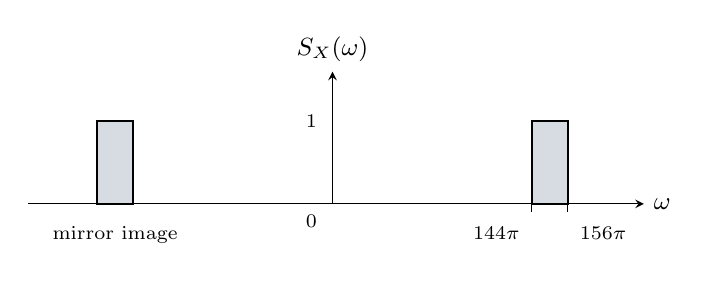
\begin{tikzpicture}[x=0.92cm,y=1.05cm,>=stealth]
  \draw[->] (-4.2,0) -- (4.3,0) node[right,font=\small] {$\omega$};
  \draw[->] (0,0) -- (0,1.6) node[above,font=\small] {$S_X(\omega)$};
  \draw[thick,fill=navy!18] (-3.25,0) rectangle (-2.75,1);
  \draw[thick,fill=navy!18] (2.75,0) rectangle (3.25,1);
  \draw[dashed] (2.75,0) -- (2.75,-0.14);
  \draw[dashed] (3.25,0) -- (3.25,-0.14);
  \node[below left,font=\scriptsize] at (2.72,-0.16) {$144\pi$};
  \node[below right,font=\scriptsize] at (3.28,-0.16) {$156\pi$};
  \node[left,font=\scriptsize] at (-0.08,1) {$1$};
  \node[below left,font=\scriptsize] at (-0.08,-0.02) {$0$};
  \node[below,font=\scriptsize] at (-3.0,-0.16) {mirror image};
\end{tikzpicture}
\end{center}
Find
\begin{qparts}
  \item the joint probability density function $f_{iq}(i,q;t,t)$;
  \item the joint probability density function $f_{iq}\!\left(i,q;t,t+\tfrac{1}{12}\right)$.
\end{qparts}\end{tcolorbox}\smallskip\begin{workspace}\hfill{\color{linec}\footnotesize Working space}\end{workspace}
\qtitle{Problem 19}{Day 7}
{\small\color{accentred}(Textbook 1.6 / Required)}\par\smallskip
{\small\color{muted}Textbook sections: 1.1.1}\par\medskip
\begin{tcolorbox}[colback=qbg,colframe=qbg,boxrule=0pt]There are four batches of components. The first batch contains $2\,000$ components, of which $5\%$ are defective. The second batch contains $500$ components, of which $40\%$ are defective. The third and fourth batches each contain $1\,000$ components, with approximately $10\%$ defective. A batch is selected at random, and then a component is drawn at random from that batch. Find:
\begin{enumerate}
\item The probability that the selected component is defective.
\item The probability that the component came from the second batch, given that it is defective.
\end{enumerate}\end{tcolorbox}\smallskip\begin{workspace}\hfill{\color{linec}\footnotesize Working space}\end{workspace}
\qtitle{Problem 20}{Day 7}
{\small\color{accentred}(Textbook 1.24 / Required)}\par\smallskip
{\small\color{muted}Textbook sections: 1.4.4}\par\medskip
\begin{tcolorbox}[colback=qbg,colframe=qbg,boxrule=0pt]The random variable $X$ is uniformly distributed on $[0,a]$. Given $X$, the random variable $Y$ is uniformly distributed on $[X,a]$. Find:
\begin{enumerate}
\item $E(Y\mid X)$, $0\leq X\leq a$;
\item $EY$.
\end{enumerate}\end{tcolorbox}\smallskip\begin{workspace}\hfill{\color{linec}\footnotesize Working space}\end{workspace}
\qtitle{Problem 21}{Day 7}
{\small\color{accentred}(Textbook 1.33 / Required)}\par\smallskip
{\small\color{muted}Textbook sections: 1.5.2}\par\medskip
\begin{tcolorbox}[colback=qbg,colframe=qbg,boxrule=0pt]The joint characteristic function of the random variables $X$ and $Y$ is
\[
\phi_{XY}(u,v)=\frac{6}{6-2\mathrm{j}u-3\mathrm{j}v-uv}.
\]
Find:
\begin{enumerate}
\item The characteristic function of $X$;
\item The expectation and variance of $Y$.
\end{enumerate}\end{tcolorbox}\smallskip\begin{workspace}\hfill{\color{linec}\footnotesize Working space}\end{workspace}
\qtitle{Problem 22}{Day 8}
{\small\color{accentred}(2018--19 Q1 (201812))}\par\smallskip
{\small\color{muted}Textbook sections: 1.3.1 / 1.6}\par\medskip
\begin{tcolorbox}[colback=qbg,colframe=qbg,boxrule=0pt]Let $X\sim U(0,1)$ and $Y=5X+1$. Find the PDF of $Y$, including its support. Check normalization.\end{tcolorbox}\smallskip\begin{workspace}\hfill{\color{linec}\footnotesize Working space}\end{workspace}
\qtitle{Problem 23}{Day 8}
{\small\color{accentred}(Adapted from 2019--20 Q1 (201912))}\par\smallskip
{\small\color{muted}Textbook sections: 1.3.1 / 1.5.1 / 1.6}\par\medskip
\begin{tcolorbox}[colback=qbg,colframe=qbg,boxrule=0pt]For this adapted question, explicitly assume $X\sim N(0,1)$ and $Y=6X+2$.
\begin{enumerate}\item Find $f_Y(y)$ and $\phi_Y(v)$.\item Explain why the original wording ``Gaussian distribution in [0,1]'' is ambiguous. If instead $X$ is a standard normal conditioned on $0\le X\le1$, give the transformed PDF and a normalized integral for its CF.\end{enumerate}\end{tcolorbox}\smallskip\begin{workspace}\hfill{\color{linec}\footnotesize Working space}\end{workspace}
\qtitle{Problem 24}{Day 8}
{\small\color{accentred}(2019--20 Q2 (201912))}\par\smallskip
{\small\color{muted}Textbook sections: 1.2.1}\par\medskip
\begin{tcolorbox}[colback=qbg,colframe=qbg,boxrule=0pt]The joint PDF is $f_{XY}(x,y)=xe^{-x(y+1)}u(x)u(y)$. Find both marginal PDFs, verify normalization, and decide whether $X$ and $Y$ are independent.\end{tcolorbox}\smallskip\begin{workspace}\hfill{\color{linec}\footnotesize Working space}\end{workspace}
\qtitle{Problem 25}{Day 9}
{\small\color{accentred}(Adapted from 2020--21 Q4(b,c) (202104))}\par\smallskip
{\small\color{muted}Textbook sections: 1.6 / 2.4.3}\par\medskip
\begin{tcolorbox}[colback=qbg,colframe=qbg,boxrule=0pt]A zero-mean stationary Gaussian input has variance $\sigma_X^2>0$ and autocorrelation $R_X(\tau)=\sigma_X^2e^{-a|\tau|}$. It passes through $h(t)=e^{-bt}u(t)$, where $a,b>0$ and $a\ne b$. You may use the Chapter 5 result
\[R_Y(\tau)=\frac{\sigma_X^2}{b^2-a^2}\left(e^{-a|\tau|}-\frac ab e^{-b|\tau|}\right).\]
Find the one-dimensional PDF of $Y(t)$ and $P\{Y(t)\ge0\}$. Explain which assumption supplies Gaussianity.\end{tcolorbox}\smallskip\begin{workspace}\hfill{\color{linec}\footnotesize Working space}\end{workspace}
\qtitle{Problem 26}{Day 9}
{\small\color{accentred}(2021--22 Q1(c) (202112))}\par\smallskip
{\small\color{muted}Textbook sections: 1.5.2 / 1.4.2}\par\medskip
\begin{tcolorbox}[colback=qbg,colframe=qbg,boxrule=0pt]Let $X(t)=A+B\cos t$, with independent $A,B\sim N(0,1)$. For $Z=(X(0),X(\pi/2))^T$, determine the covariance matrix and the joint characteristic function $\phi_Z(u,v)$. Are the components independent?\end{tcolorbox}\smallskip\begin{workspace}\hfill{\color{linec}\footnotesize Working space}\end{workspace}
\qtitle{Problem 27}{Day 9}
{\small\color{accentred}(Textbook 1.9 / Optional)}\par\smallskip
{\small\color{muted}Textbook sections: 1.1.2}\par\medskip
\begin{tcolorbox}[colback=qbg,colframe=qbg,boxrule=0pt]The random variable $X$ has the following probability mass function:
\begin{center}
\renewcommand{\arraystretch}{1.35}
\begin{tabular}{c|ccc}
\toprule
$X$ & $1$ & $2$ & $3$ \\
\midrule
$P$ & $0.2$ & $0.5$ & $0.3$ \\
\bottomrule
\end{tabular}
\end{center}
Find the probability density function and distribution function of $X$, and sketch their graphs.\end{tcolorbox}\smallskip\begin{workspace}\hfill{\color{linec}\footnotesize Working space}\end{workspace}
\qtitle{Problem 28}{Day 10}
{\small\color{accentred}(Textbook 1.11 / Optional)}\par\smallskip
{\small\color{muted}Textbook sections: 1.1.2}\par\medskip
\begin{tcolorbox}[colback=qbg,colframe=qbg,boxrule=0pt]The random variable $X$ has probability density function $f(x)=a\mathrm{e}^{-|x|}$. Find:
\begin{enumerate}
\item The coefficient $a$;
\item Its distribution function.
\end{enumerate}\end{tcolorbox}\smallskip\begin{workspace}\hfill{\color{linec}\footnotesize Working space}\end{workspace}
\qtitle{Problem 29}{Day 10}
{\small\color{accentred}(Textbook 1.28 / Optional)}\par\smallskip
{\small\color{muted}Textbook sections: 1.5.1}\par\medskip
\begin{tcolorbox}[colback=qbg,colframe=qbg,boxrule=0pt]The random variables $X_1,X_2,X_3$ are mutually independent, with characteristic functions $\phi_1(v)$, $\phi_2(v)$, and $\phi_3(v)$, respectively. Find the characteristic function of each of the following random variables:
\begin{enumerate}
\item $X=X_1+X_2$;
\item $X=X_1+X_2+X_3$;
\item $X=X_1+2X_2+3X_3$;
\item $X=2X_1+X_2+4X_3+10$.
\end{enumerate}\end{tcolorbox}\smallskip\begin{workspace}\hfill{\color{linec}\footnotesize Working space}\end{workspace}
\qtitle{Problem 30}{Day 10}
{\small\color{accentred}(Textbook 1.30 / Optional)}\par\smallskip
{\small\color{muted}Textbook sections: 1.5.1}\par\medskip
\begin{tcolorbox}[colback=qbg,colframe=qbg,boxrule=0pt]Use the Fourier transform to derive the characteristic function of the uniform distribution.\end{tcolorbox}\smallskip\begin{workspace}\hfill{\color{linec}\footnotesize Working space}\end{workspace}
\end{document}